\documentclass{article}

\usepackage{amsmath}
\usepackage{amssymb}
\usepackage{graphicx}
\usepackage[spanish]{babel}
\usepackage{cancel}
\usepackage{enumerate}
\usepackage{hyperref}
\hypersetup{
    colorlinks,
    citecolor=black,
    filecolor=black,
    linkcolor=black,
    urlcolor=black,
}
\usepackage{tcolorbox}
\usepackage{xcolor}

\tcbuselibrary{theorems}

\newcommand{\hresult}[2]{\tcboxmath[colback=orange!25!white,colframe=orange, title=#1] {#2} }
\newcommand{\hresulte}[3]{\tcboxmath[colback=orange!25!white,colframe=orange, title=#1] { \hspace{#3} #2 \hspace{#3} } }

\renewcommand{\Bbb}{\mathbb}

\title{Ejercicios de Análisis Matemático CBC (28) \\
Práctica 1: Funciones reales \\
Cátedra Ruiz, curso 62802 \\
1° C 2003}
\author{Darío Eduardo Ramos}

\begin{document}
\maketitle

\tableofcontents{}

\newpage

\section*{1}
\label{sec:1}
\addcontentsline{toc}{section}{\nameref{sec:1}}

\textbf{Haga un gráfico que refleje la evolución de la temperatura del agua a lo largo del tiempo atendiendo a la siguiente descripción:}

\vspace{1em}

\textbf{``Saqué del fuego una cacerola con agua hirviendo. Al principio, la temperatura del agua bajó con rapidez, de modo que a los 5 minutos estaba en 60º. Luego fue enfriándose con más lentitud. A los 20 minutos de haberla sacado estaba a 30º y 20 minutos después seguía teniendo algo más de 20º, temperatura de la cual no bajó, pues era la temperatura que había en la cocina.'' }

\vspace{1em}

\textbf{¿Es el gráfico que hizo el único que respeta las consignas anteriores?}

\vspace{1em}

\hrule

\vspace{1em}

Planteando la temperatura como una función del tiempo, llámese $y = f(t)$, los datos que se tienen sobre $f$ son los siguientes:

\begin{subequations}
\begin{align}
& f(t < 0) = 100 \\
& f(0) = 100 \\
& f(5) = 60 \\
& f(20) = 30 \\
& f(40) = 20+ \\
& f(t > 40) = 20
\end{align}
\end{subequations}

Dado que no se tiene una expresión cerrada para $f$, existen infinitas funciones de variable continua que satisfacen estas restricciones. Cualquier gráfico que se haga que pase por los puntos dados y se mantenga constante para $t < 0$ y $t > 40$ con los valores dados es válido. Resulta conveniente definir los grados Celsius como la unidad del eje $y$, y los minutos como la unidad del eje $x$. Por ejemplo:

\newpage

\begin{figure}[ht]
\caption{un gráfico posible}
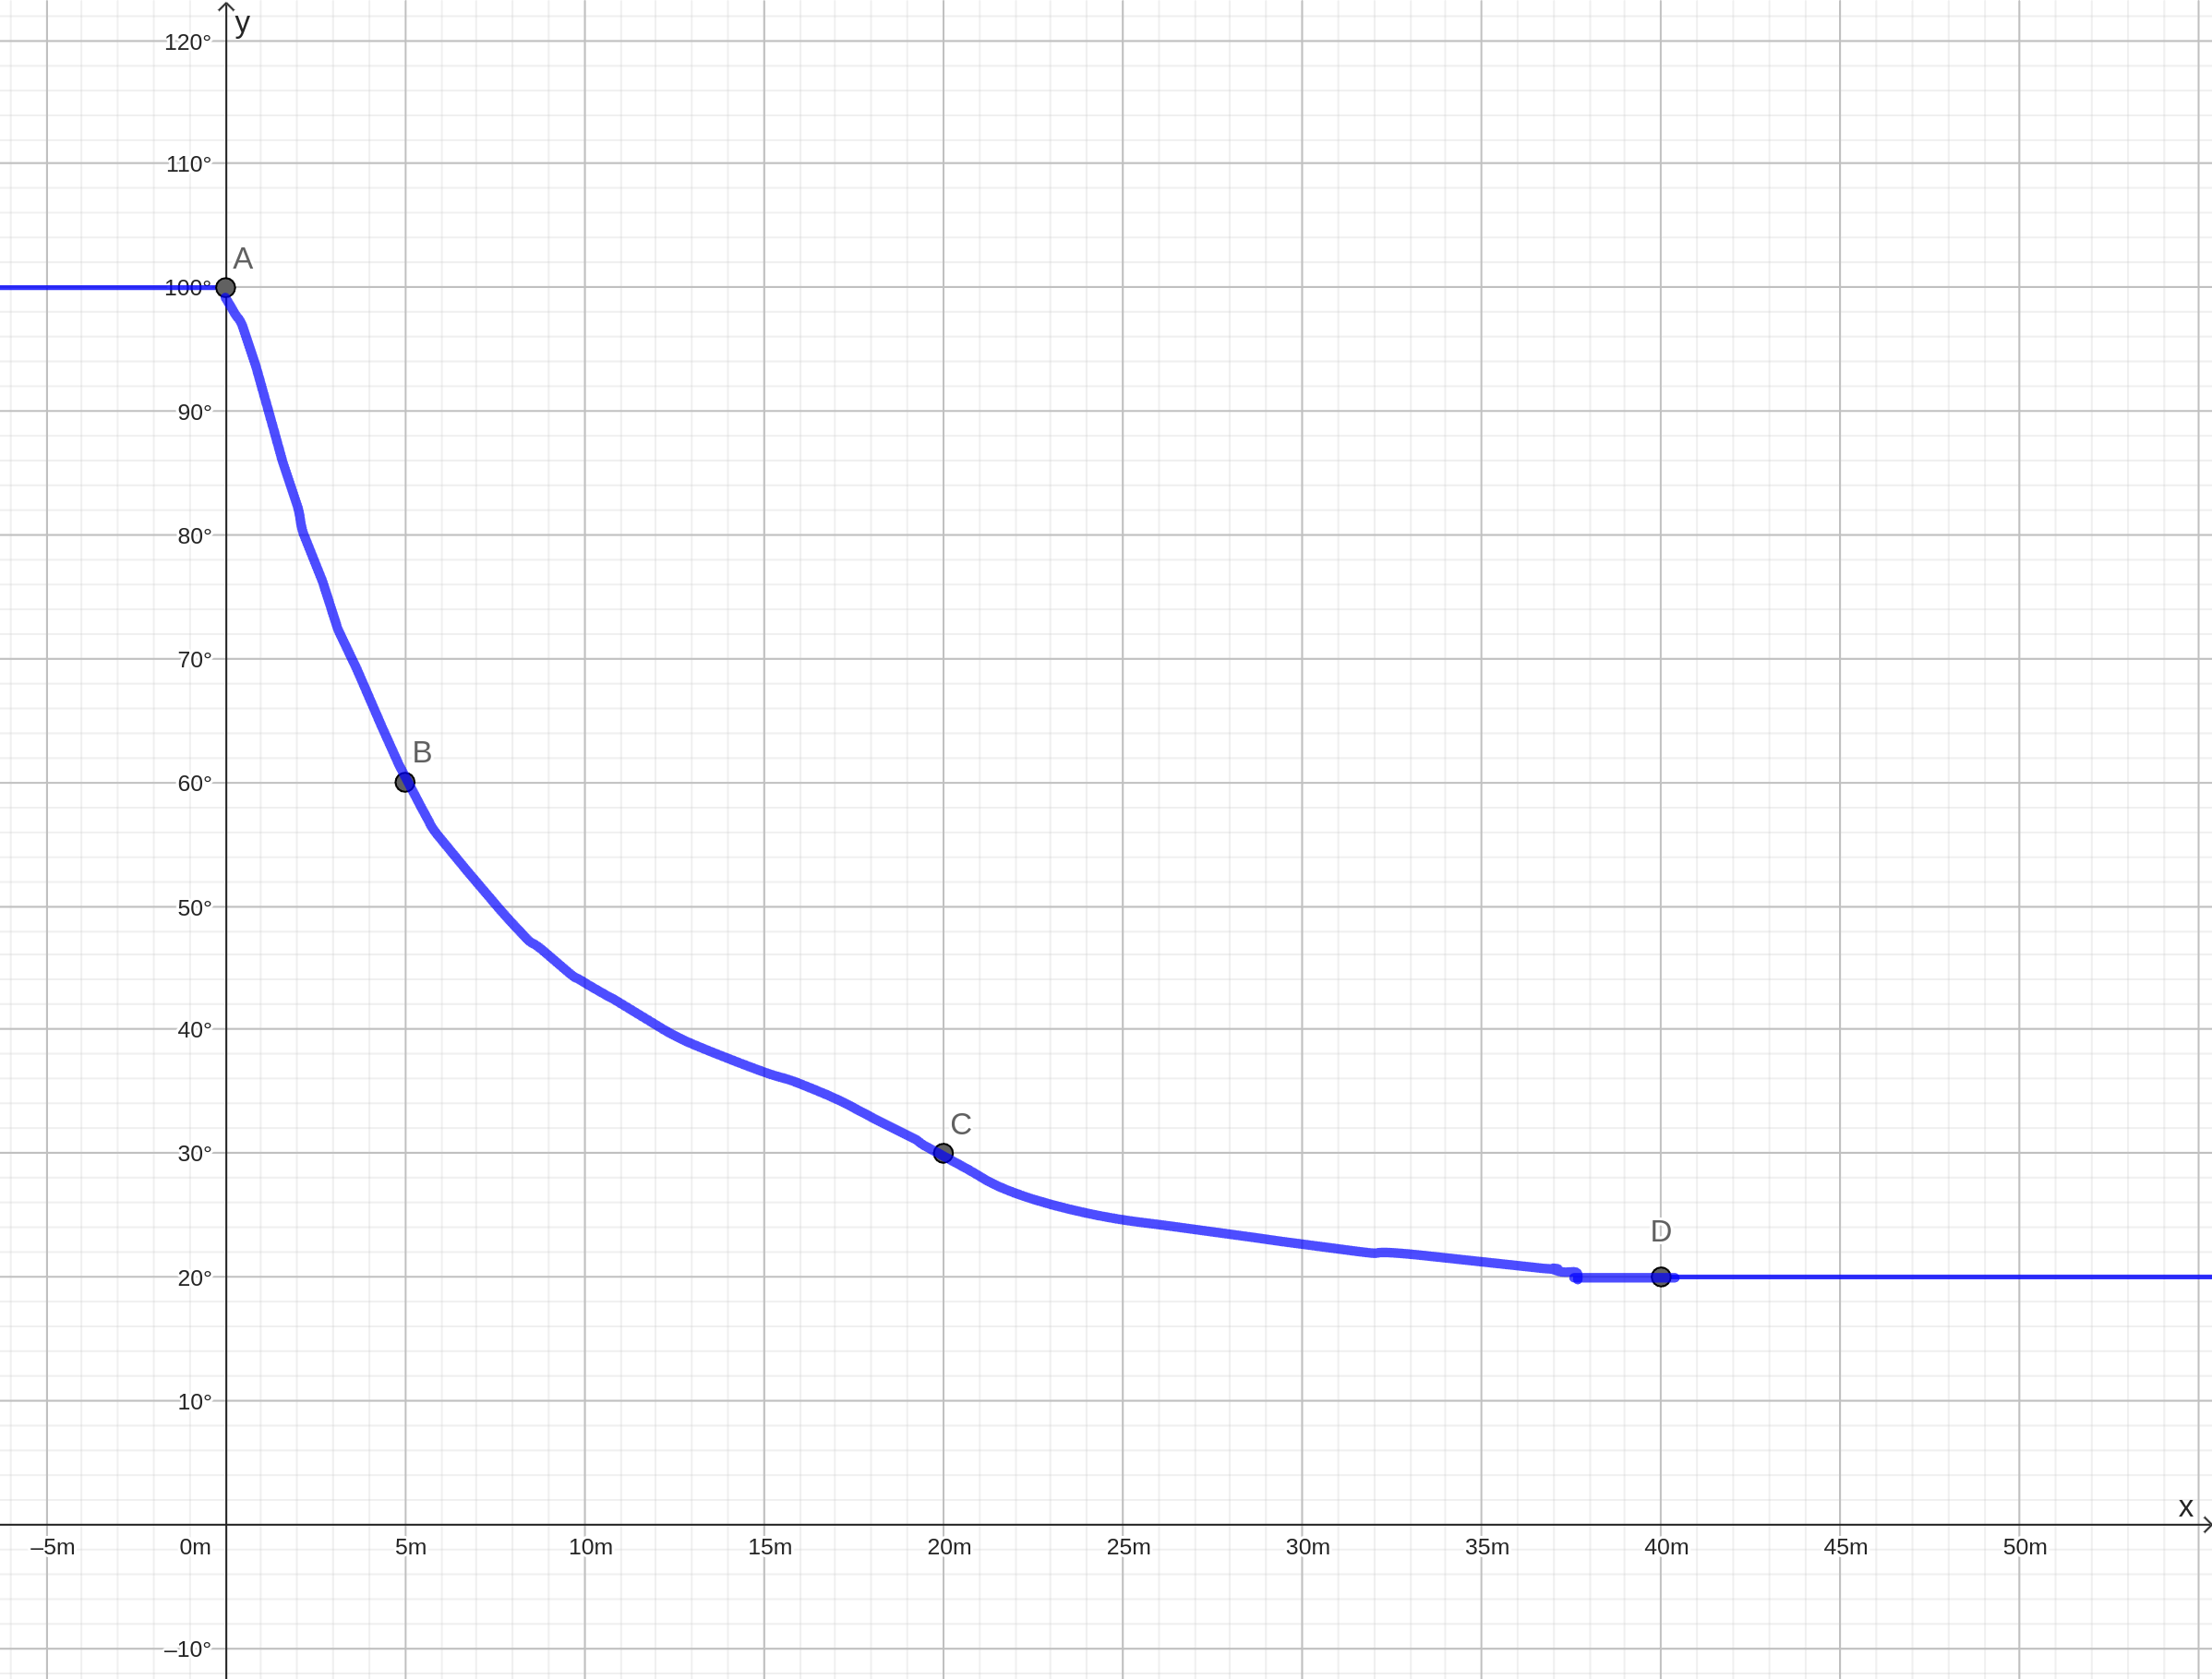
\includegraphics[scale=0.17]{../img/guide_01/ex_01.png} 
\centering
\label{fig:1}
\end{figure}

\section*{2}
\label{sec:2}
\addcontentsline{toc}{section}{\nameref{sec:2}}

\textbf{Con una lámina rectangular de 40 por 30 queremos hacer una caja como muestra la figura~\ref{fig:2}}

\begin{figure}[ht]
\caption{}
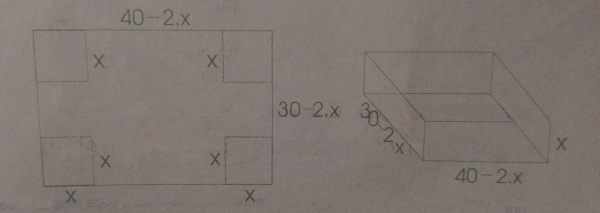
\includegraphics[scale=2]{../img/guide_01/ex_02.png} 
\centering
\label{fig:2}
\end{figure}

\begin{enumerate}[(a)]

\item \textbf{Busque la expresión del volumen de la caja en función de $x$. }

\item \textbf{¿Cuál es el dominio?}

\item \textbf{Haga un gráfico aproximado a partir de una tabla de valores.}

\end{enumerate}
\hrule

\subsection*{2.a}
\label{subsec:2.a}
\addcontentsline{toc}{subsection}{\nameref{subsec:2.a}}

El volumen de un cubo no regular, u ortoedro o prisma rectangular, es el área de su base multiplicada por su altura. En este caso:

\begin{equation}
v(x) = (30-2x)(40-2x)x = \hresult{2.a}{ 4x^3 - 140x^2 +1200x }
\end{equation}

\subsection*{2.b}
\label{subsec:2.b}

Exigiendo que todos los lados sean mayores a cero, se obtiene:

\begin{subequations}
\begin{align}
& 30 - 2x > 0 \Rightarrow 30 > 2x \Rightarrow x < 15 \\
& 40 - 2x > 0 \Rightarrow 40 > 2x \Rightarrow x < 20 \\
& x > 0
\end{align}
\end{subequations}

Para que estas tres condiciones se cumplan al mismo tiempo, debe ser:

\begin{equation}
\hresult{2.b}{ \mathop{\text{Dom}}(v) = \{ x \in \mathbb{R} / 0 < x < 15 \} }
\end{equation}

\subsection*{2.c}
\label{subsec:2.c}

La función $v(x)$ es cúbica, con ceros en 0, 15 y 30. Cabe esperar un máximo en el dominio definido, ya que $v(0) = v(15) = 0$.

\begin{center}
\begin{tabular}{||c c||} 
 \hline
 x & v(x) \\ [0.5ex] 
 \hline\hline
 1 & 1064 \\ 
 \hline
 3 & 2448 \\
 \hline
 5 & 3000 \\
 \hline
 7 & 2912 \\
 \hline
 9 & 2376 \\
 \hline
 11 & 1584 \\
 \hline
 13 & 728 \\ [1ex] 
 \hline
\end{tabular}
\end{center}

\newpage

\begin{figure}[ht]
\caption{}
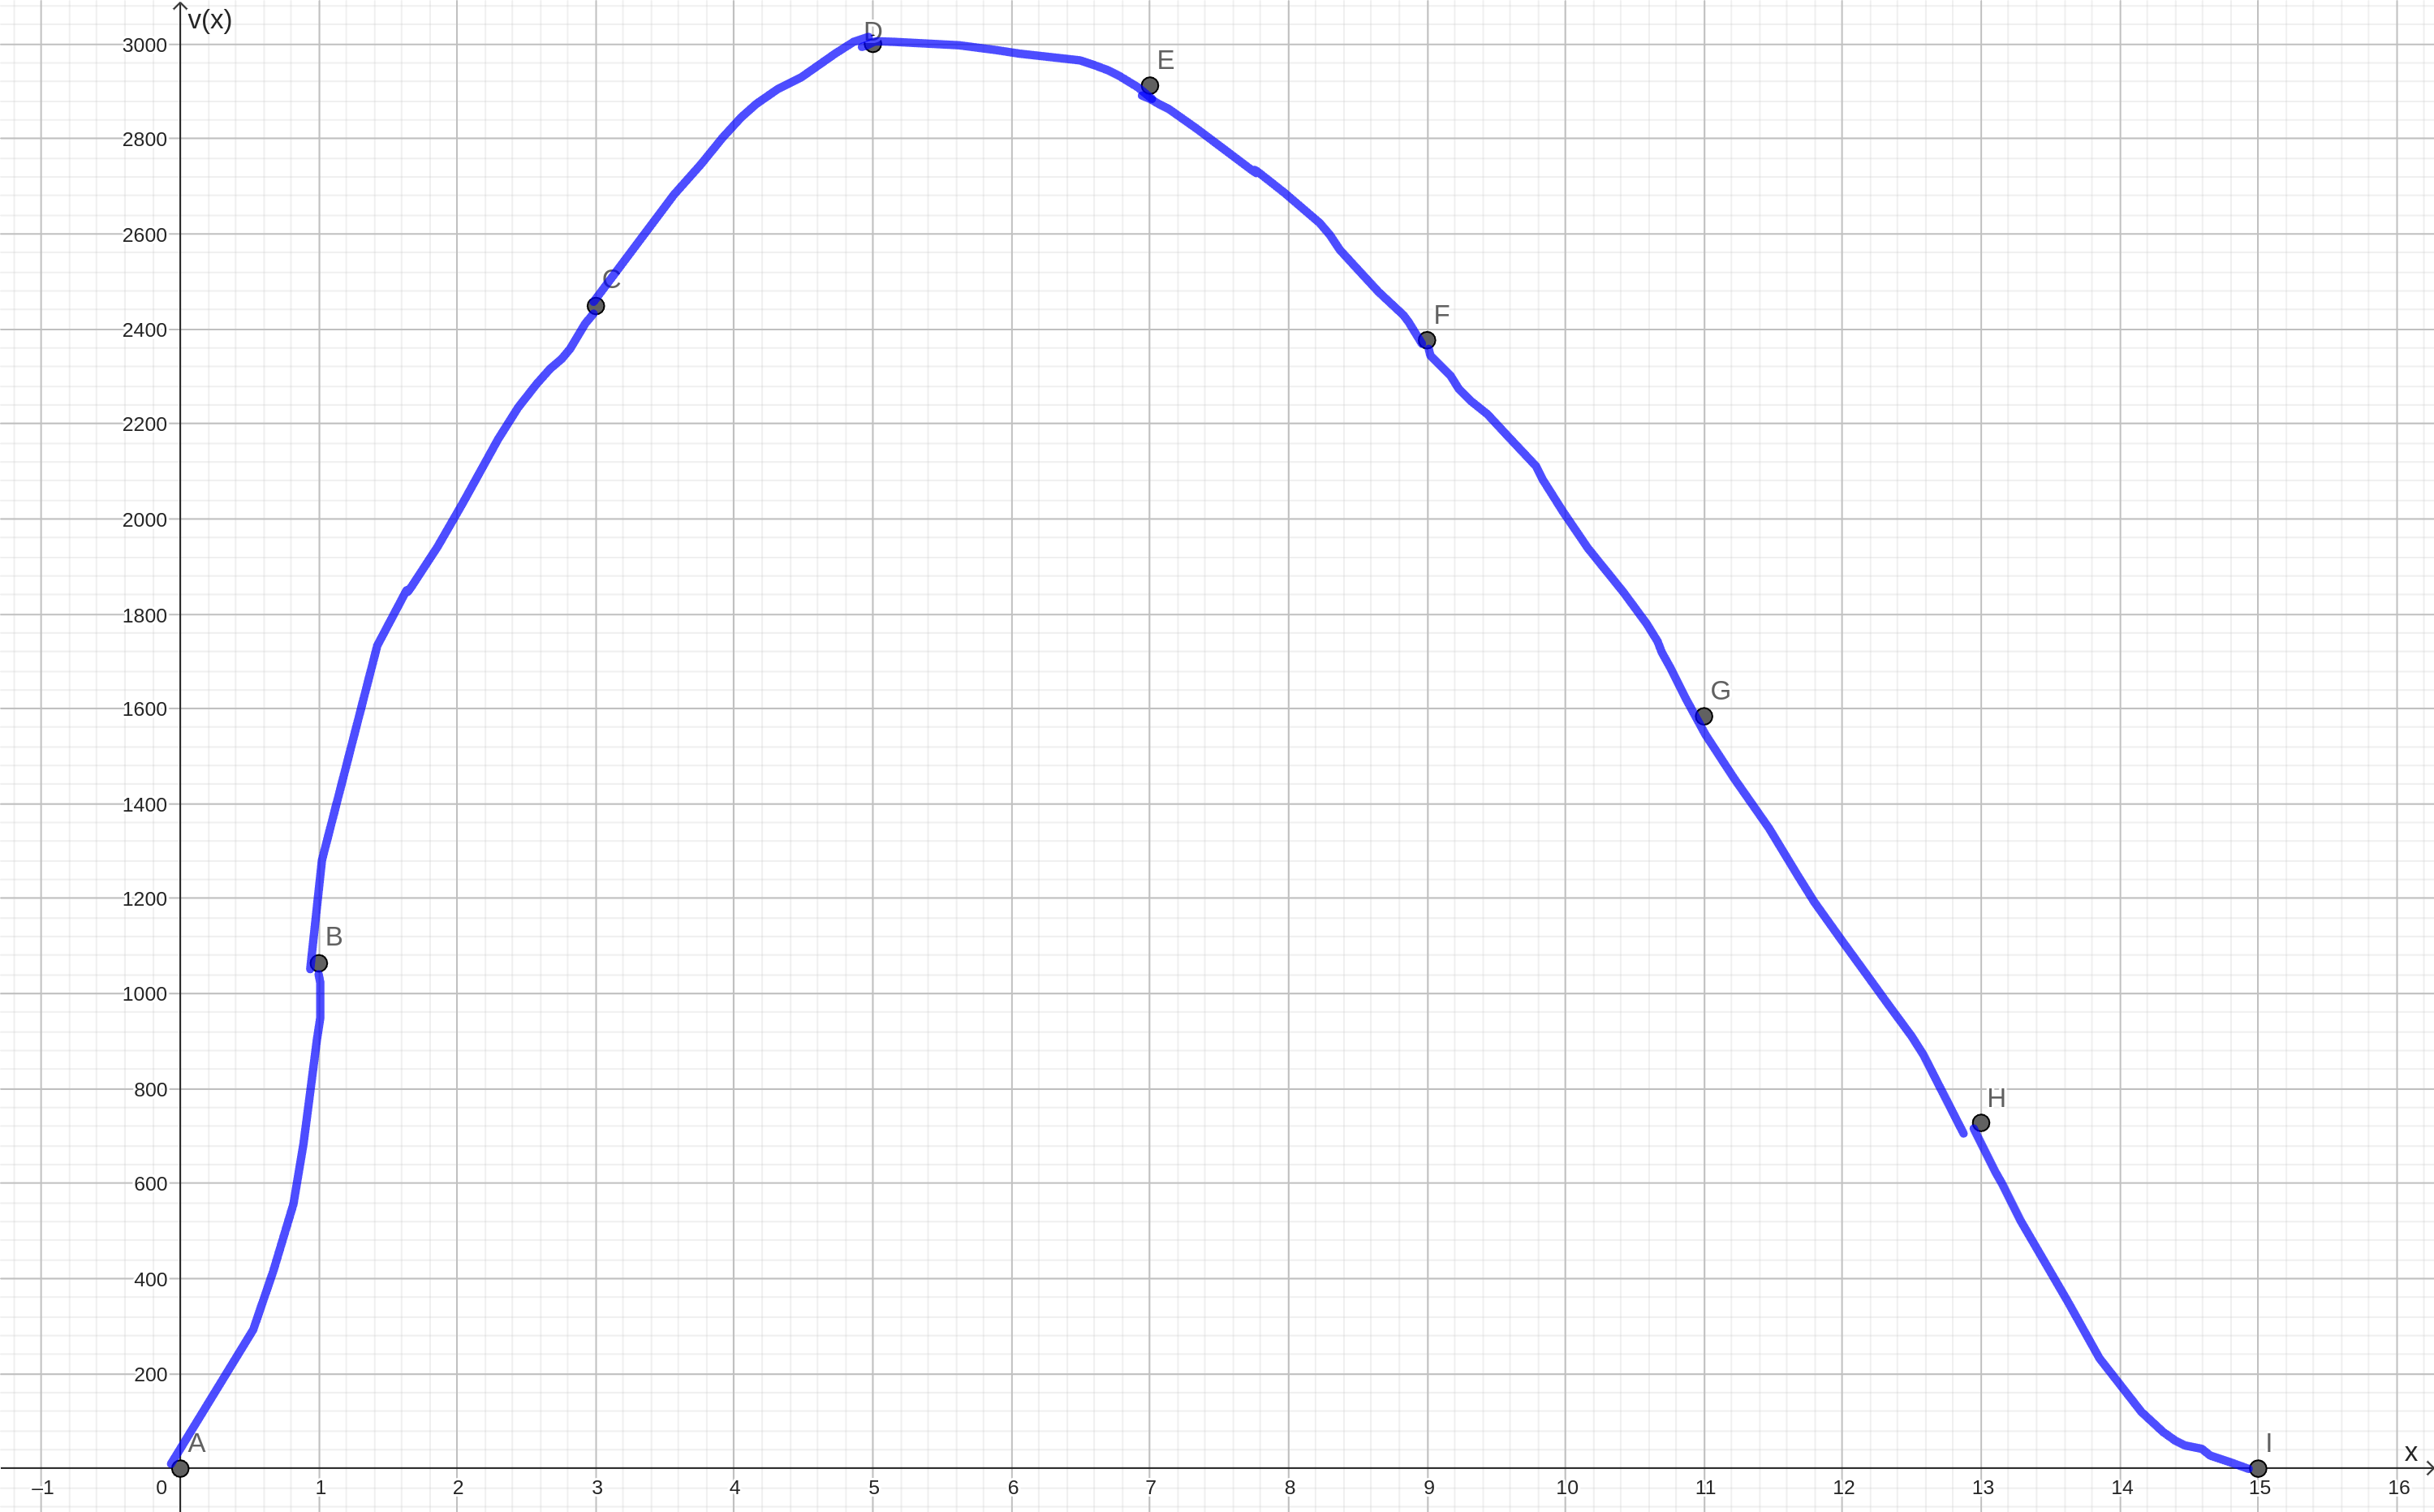
\includegraphics[scale=0.6]{../img/guide_01/ex_02c.png} 
\centering
\label{fig:2c}
\end{figure}

\section*{3}
\label{sec:3}
\addcontentsline{toc}{section}{\nameref{sec:3}}

\textbf{Entre todos los rectángulos de perímetro 20, halle la función que relaciona la base $x$ con la altura $y$. Haga un gráfico que la represente. ¿Cuál es el dominio?}

\vspace{1em}
\hrule
\vspace{1em}

El perímetro es la suma de los lados. Si la base es $x$ y la altura es $y$, el perímetro es:

\begin{equation}
P = x + x + y + y
\end{equation}

Dado que el perímetro es siempre 20:

\begin{equation}
20 = 2x + 2y
\end{equation}

Despejando y:

\begin{equation}
y = 10 - x
\end{equation}

Para obtener el dominio, se exige que tanto $x$ como $y$ sean positivos. Dado que $y$ depende de $x$, resulta $10 - x > 0 \Rightarrow x < 10$. El dominio es entonces:

\begin{equation}
\hresult{Dominio}{ \mathop{\text{Dom(y)}} = \{ x \in \mathbb{R} / 0 < x < 10 \} }
\end{equation}

\newpage

\begin{figure}[ht]
\caption{Gráfico de y = 10-x}
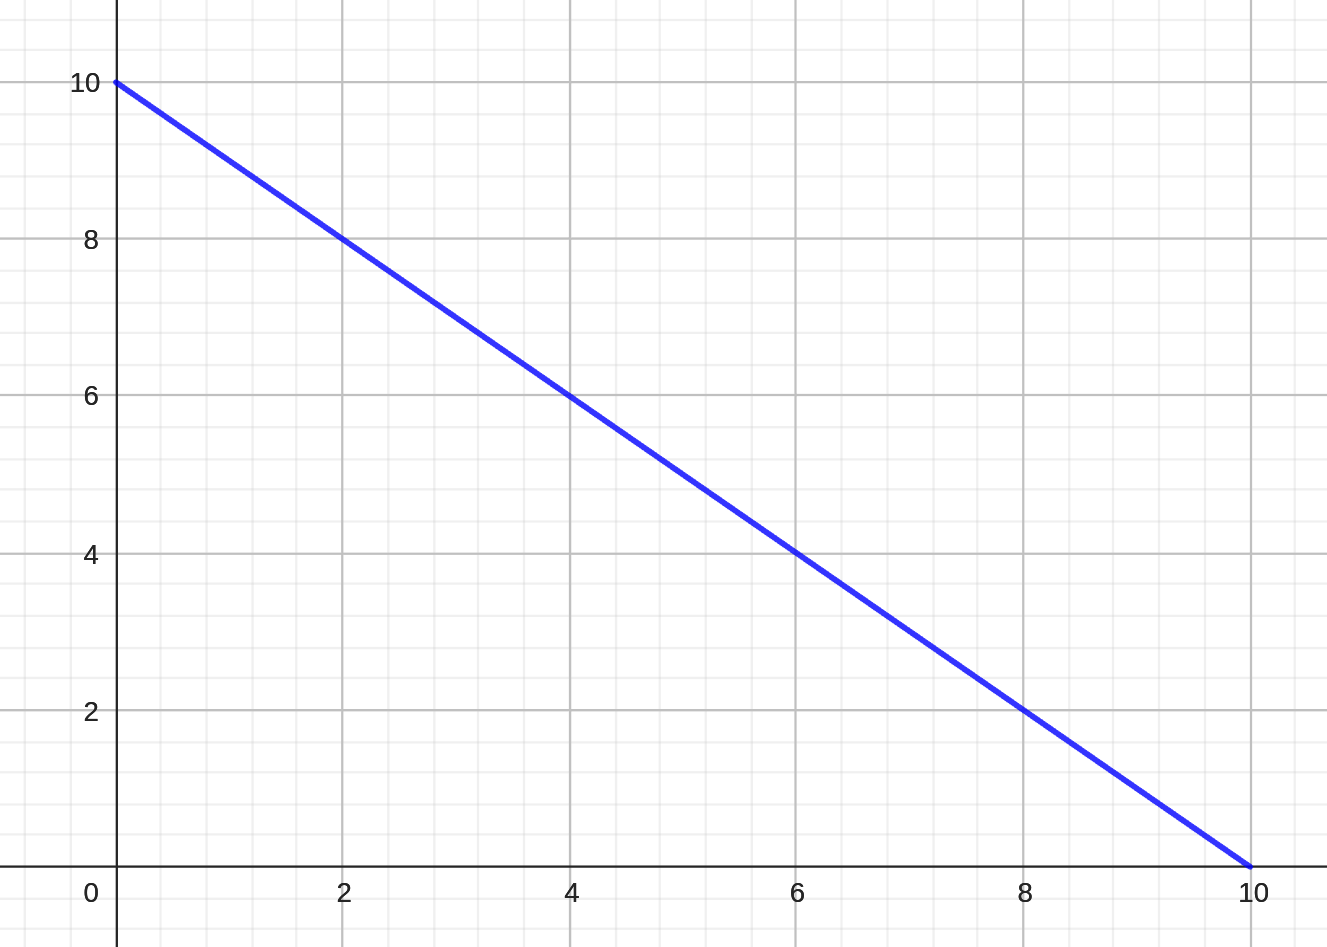
\includegraphics[scale=0.8]{../img/guide_01/ex_03.png} 
\centering
\label{fig:3}
\end{figure}

\section*{4}
\label{sec:4}
\addcontentsline{toc}{section}{\nameref{sec:4}}

\textbf{Halle el área de un triángulo rectángulo isósceles en función del cateto. Dibuje el gráfico de la función hallada a partir de una tabla de valores. Indique cuál es el dominio.}

\vspace{1em}
\hrule
\vspace{1em}

Si un cateto mide $x$, por ser isósceles el otro cateto también mide $x$. Dado que el área de un triángulo es base por altura sobre dos, tomando un cateto como base y el otro como altura, resulta:

\begin{equation}
\hresult{4}{ a(x) = \frac{x^2}{2}, \mathop{\text{Dom}}(a) = \{ x \in \mathbb{R} / x > 0 \} }
\end{equation}

\newpage

\begin{figure}[ht]
\caption{Gráfico de $y = x^2/2 $}
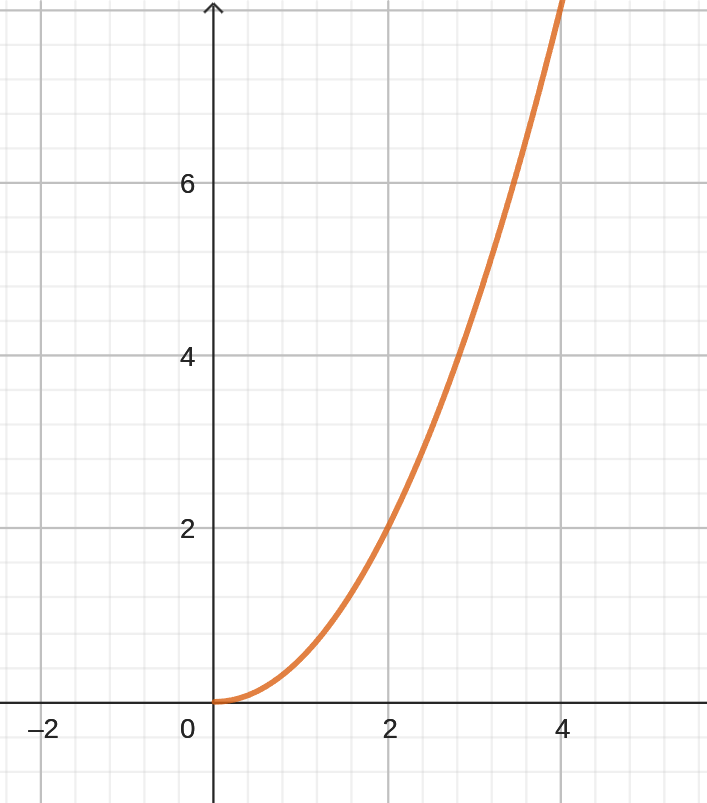
\includegraphics[scale=0.8]{../img/guide_01/ex_04.png} 
\centering
\label{fig:4}
\end{figure}\textbf{•}

\section*{5}
\label{sec:5}
\addcontentsline{toc}{section}{\nameref{sec:5}}

\textbf{Dados los siguientes conjuntos del plano, determine, en cada caso, si existe una función cuyo gráfico sea el dado.}

\begin{figure}[ht]
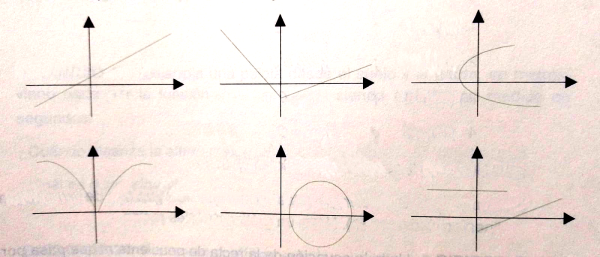
\includegraphics[scale=2]{../img/guide_01/ex_05.png} 
\centering
\label{fig:5}
\end{figure}

\hrule
\vspace{1em}

Etiquetando de izquierda a derecha (a, b y c son la primera fila y d, e y f la segunda):

\begin{enumerate}[(a)]
\item Sí, es una recta con pendiente positiva. Puede verse como una función de $x$ y también como una función de $y$.

\item Sí, aunque sólo como función de $x$. Si se ve como función de $y$, hay valores de $y$ para los cuales hay más de un valor de $x$. Esto rompe la propiedad de unicidad de las funciones. Volviendo al caso válido, $y = f(x)$ puede armarse como una función por partes. Para $x < 0$, es una recta con pendiente negativa, y para $x > 0$, pendiente positiva. Ambas cortan al eje $y$ en el mismo punto.

\item No como función de $x$, pero sí como función de $y$. En este segundo caso, puede ser una parábola de la forma $x = a (y-y_0)^2 + b$

\item Sí como función de $x$, no como función de $y$. En el caso válido, puede armarse como una rama parabólica para $x < 0$ y otra para $x > 0$. Ambas cortarían al eje $y$ en cero.

\item No, ni como función de $x$ ni como función de $y$. En ambos casos la variable independiente puede tener múltiples valores de variable dependiente asociada. Aunque no se pueda definir una función para este conjunto, dado que es un círculo, puede ser definido por una expresión de la forma $ (x-x_0)^2 + (y-y_0)^2 = r^2$. Con esta notación, el punto $(x_0, y_0)$ es el centro del círculo, y $r$ su radio.

\item No, ni como función de $x$ ni como función de $y$. En ambos casos se rompe la unicidad.

\end{enumerate}

\section*{6}
\label{sec:6}
\addcontentsline{toc}{section}{\nameref{sec:6}}

\textbf{Dados los siguientes gráficos de funciones, determine, en cada caso, en qué intervalos es creciente, en qué intervalos es decreciente, en qué punto alcanza su máximo, cuál es dicho valor máximo, en qué punto alcanza su mínimo y cuál es el valor mínimo.}

\begin{figure}[ht]
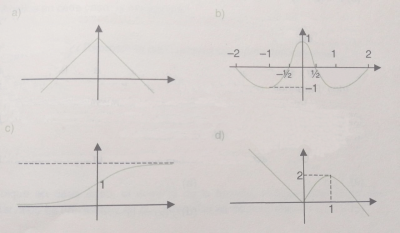
\includegraphics[scale=3]{../img/guide_01/ex_06.png} 
\centering
\label{fig:6}
\end{figure}

\subsection*{6.a}
\label{subsec:6.a}

\begin{itemize}

\item IC: $(-\infty, 0)$

\item ID: $(0, +\infty)$

\item Máximo: Se alcanza en $x = 0$, y es $f(0)$ (no se indica el valor exacto en el gráfico).

\item Mínimo: $\nexists$

\end{itemize}

\subsection*{6.b}
\label{subsec:6.b}

\begin{itemize}

\item IC: $(-1, 0) \cup (1, 2)$

\item ID: $(-2, -1) \cup (0, 1)$

\item Máximo: $1$, se alcanza en $x = 0$

\item Mínimo: $-1$, se alcanza en $x = -1$ y $x = 1$.

\end{itemize}

\subsection*{6.c}
\label{subsec:6.c}

\begin{itemize}

\item IC: $(-\infty, +\infty)$

\item ID: $\emptyset$

\item Máximo: $\nexists$

\item Mínimo: $\nexists$

\end{itemize}

Nótese que a pesar de estar acotada, esta función no tiene mínimo ni máximo porque se comporta asintóticamente. Con x tendiendo a menos infinito, tiende a cero pero nunca lo alcanza. Y lo mismo ocurre con más infinito y 1.

\subsection*{6.d}
\label{subsec:6.d}

\begin{itemize}

\item IC: $(0, 1)$

\item ID: $(-\infty, 0) \cup (1, +\infty)$

\item Máximo: $\nexists$

\item Mínimo: $\nexists$

En este caso, no hay mínimo ni máximo porque la función no está acotada. Sin embargo, tiene un mínimo local en $x = 0$ y un máximo local en $x = 1$.

\end{itemize}

\end{document}
